\begin{savequote}[8cm]
Why genes in pieces?
  \qauthor{--- Walter Gilbert \cite{whygenesinpieces}, in response to the discovery of splicing}
\end{savequote}

\chapter{\label{ch:1-intro}Introduction} 
"One gene, one protein" was the prevailing dogma for over 30 years. Yet this belief was turned upside down by the stunning discovery in 1977 that genes contain long non-coding sequences \cite{discoveryofsplicing} (see Figure \ref{fig:discovery}). Instead, these non-coding sequences (introns) must be removed and only the coding sequences (exons) are joined together to form the blueprint of a gene product. Different sequences may be spliced together in different ways under different circumstances, allowing one gene to encode multiple proteins. Splicing and Alternative Splicing were discovered. 

%Gene expression is fundamental to all life. It is the process whereby a sequence of nucleotides is used to direct the synthesis of a functional gene product (protein, functional RNA). And even though gene expression is such a fundamental process, our understanding of it is still lacking [alzheimer, dark matter]. 
%
%Since the discovery of genes[TODO], it was believed that the entire sequence is dedicated to encoding functional gene products \cite{onegeneoneprotein}. The dogma was one gene, one protein. Yet this belief was turned upside down by a stunning finding in 1977 that genes contain long non-coding sequences \cite{discoveryofsplicing} [figure]. Instead, these non-coding sequences must be removed and only the coding sequences are joined together to make the blueprint of a gene product. Splicing was discovered. 

\begin{figure}
	\centering
%	\frame{
		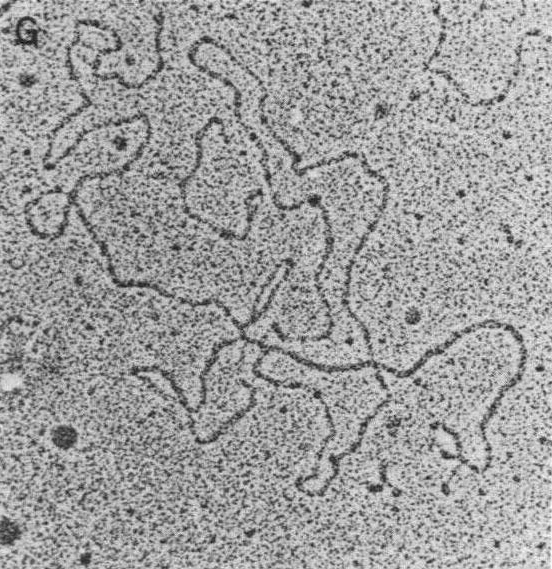
\includegraphics[width=0.49\textwidth]{../visualizations/ch1-introduction/original_electron_microscopy.jpg}
%	} 
	\frame{ 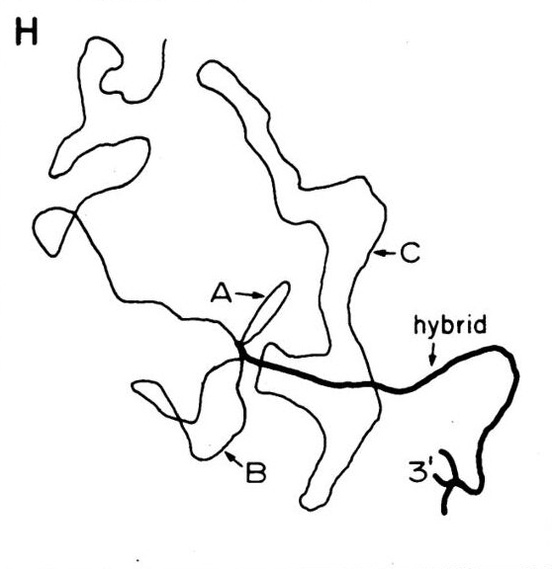
\includegraphics[width=0.49\textwidth]{../visualizations/ch1-introduction/schematic_electron_microscopy.jpg}
	}
	\caption{Original electron microspy leading to the discovery of splicing (left) and schematic (right) \cite{discoveryofsplicing}. Introns show up as loops in this image.  }
	\label{fig:discovery}

\end{figure}

But "Why genes in pieces?". This question was posed by Walter Gilbert one year later \cite{whygenesinpieces}. Gilbert answered his own question and proposed that splicing, in essence, provides a multiplier which speeds up the rate of evolutionary adaption: a single nucleotide mutation influencing splicing may now lead to the inclusion or exclusion of whole genomic regions and thus the generation of a novel gene product. Was Gilbert correct? 42 years later we are still uncertain, but some support for his ideas have been found \cite{whyrevisited}. %perhaps introduction of alternative splicing

What we have gained in the past four decades of research, is a greater appreciation of the importance and the complexity of splicing. 
Misregulated alternative splicing is a biomarker for several forms of cancer \cite{cancer} \cite{splicingcausescancer} and up to 50\% of known disease-causing mutations in humans have been shown to affect splicing \cite{50diseasessplicing}. 
Yet, our understanding of splicing is still limited: the core splicing signals which we have found are estimated to only account for approximately 50\% of splicing behaviour even in limited circumstances \cite{coresplicingsignals50percentexplainit}. The remaining 50\% are likely accounted for by the complex interactions of numerous cis-regulatory elements. 

An important long-term goal is the development of a splicing code which describes the regulatory mechanisms governing splicing and unifies them into a predictive model \cite{longtermcall}. Due to splicing's complexity, attempts at these splicing codes have been increasingly based on computational models \cite{barash2010a} and although many have been proposed, they are still too simplistic to explain the complex splicing behaviour we observe. %fail to explain a lot of the splicing behaviour we observe. %TODO ask liz/will whether this is true 

%attempts at formulating a splicing code have been increasingly computational. 


%What we search for is a splicing code .. which describes the regulatory mechanisms underlying splicing 
%
%This greater appreciation for the complexity of splicing, has lead to a long-term call to develop computational splicing codes which can model the complex interactions regulating splicing. 
%a decade ago
%
%although many such splicing codes have been proposed, they still fail to account for much of the regulation in splicing their 


% determine a set of rules which will determine the splicing of a gene from its sequence


%'Thus, in addition to predictive accuracy, faithfulness to the in vivo mechanism is important in splicing simulation, and an important application of splicing simulation is to evaluate how different sequence features contribute to the determination of splicing specificity.' 

% this is great actually, can point to it when I say how lengths shouldn't be used 

%https://www.ncbi.nlm.nih.gov/pmc/articles/PMC2327353/ long term call article... 



%`silent' DNA
% introns - intragenic regions
% exons - expressed regions
% majority of DNA is in introns --> make use of this
% exons held in a matrix of silent DNA
% splicing is a multiplier for the rate of evolutionary adaption because single nucleotide changes can now lead to the inclusion or exlusion of whole genomic regions
% much faster generation of new proteins possible

% old functions does not need to be destroyed because both transcript versions can still be synthesized; no duplication of the first gene in the first place necessary
% dogma of one gene, one polypeptide chain disappears


A parallel development has been the rise of deep learning fuelled by increasing data availability and the development of powerful GPUs \cite{deeplearning}. 
Originating from Computer Vision \cite{alexnet}, deep learning has brought about breakthroughs in tasks as disparate as the early detection of Alzheimer's disease \cite{alzheimerdeeplearning} or estimating the demographic makeup of the US \cite{demographic}. 
%deep learning also hasn't missed biology and, in particular, genomics. 
%It has been applied to the prediction of protein structure [alphafold]
With the advent of next-generation sequencing, the amount of genomic data available has increased by a multi-fold making genomics a prime application domain for deep learning. 

%deep learning has produced breakthroughs in the ability of machines to interpret images, text and audio. 


Our work lies at the intersection between the desire for better splicing codes and the revolution of many fields by deep learning. We develop a Recurrent Attentive Splicing Code (RASC) inspired by deep learning techniques known from Natural Language Processing (NLP). During evaluation, we find that we can replicate the performance of a 20,000 parameter splicing model using a 100 parameter model which takes no sequence information as input when reusing a dataset by the literature. Motivated by this finding, we set out to develop better datasets and construct datasets based on three different processing methods. We show that only one of them provides appropriate data quality and quantity for the training of deep learning-based splicing codes. Comparing RASC against two reimplemented splicing codes, we show that it outperforms the previous state-of-the-art splicing code for alternative splicing exon classification by 15\%. 


%In summary, we our main contributions are as follows:
%\begin{itemize}
%	\item we show that a dataset used in previous research is critically confounded.
%	\item we construct a new dataset to train Machine Learning-based splicing codes.
%	\item we develop a new state-of-the-art splicing code.
%\end{itemize}


%\section{Document structure}
The rest of the text is organized as follows:
\begin{itemize}
	\item Chapter 2 succinctly introduces the required biological background required to follow the rest of this work. It also gives more detail about the importance of splicing.
	\item Chapter 3 reviews the splicing codes which have already been developed.
	\item Chapter 4 describes the dataset construction and the evaluated models in detail. It is by far the longest and most theoretical chapter due to us developing datasets and due to us modifying the attention mechanism known from Transformer models.
	\item Chapter 5 presents the results of evaluating the models on a total of 16 different datasets. This includes the dataset whom we show to be critically confounded and the datasets for whose future us we advocate.
	\item Chapter 6 summarizes our findings and draws more general conclusions. We also give suggestions for future work.
\end{itemize}
%\minitoc